\documentclass[runningheads,a4paper]{llncs}
\usepackage[T1]{fontenc}
\usepackage{newtxtext}
\usepackage[varvw]{newtxmath}
\usepackage{amsmath}
\usepackage{graphicx}
\usepackage{booktabs}
\usepackage{array}
\usepackage{marvosym}
\usepackage{cite}
\usepackage[hidelinks]{hyperref}
\renewcommand\UrlFont{\rmfamily}
\urlstyle{rm}
\newcolumntype{L}[1]{>{\raggedright\arraybackslash}p{#1}}
\newcommand{\pmsd}[2]{#1\,$\pm$\,#2}
\renewcommand{\topfraction}{0.9}
\renewcommand{\bottomfraction}{0.8}
\renewcommand{\textfraction}{0.1}
\renewcommand{\floatpagefraction}{0.85}
\setcounter{topnumber}{3}
\setcounter{totalnumber}{4}
% Settings chosen on the inner split (Sect. 3.4); one place for each value.
% The chosen settings (\topoweight, \cellwidth, \burstq, \windowsec, \supportq, \noveltyq) come from generated/numbers.tex.
\newcommand{\OursMean}{0.991}
\newcommand{\RawMean}{0.979}
\newcommand{\OursSd}{0.004}
\newcommand{\RawSd}{0.001}
\newcommand{\GainMin}{0.008}
\newcommand{\GainMax}{0.017}
\newcommand{\BootstrapIntervals}{[0.006, 0.010], [0.015, 0.020], [0.009, 0.013]}
\newcommand{\BestBaselineMean}{0.975}
\newcommand{\DetectorMean}{0.990}
\newcommand{\DetectorSd}{0.004}
\newcommand{\TestBenignOutside}{2{,}125}
\newcommand{\TestBenignOutsideLoic}{1{,}667}
\newcommand{\LoicRequestDetection}{99.01}
\newcommand{\LoicNoReplyDetection}{0.28}
\newcommand{\NoCorrMean}{0.965}
\newcommand{\RawCorrMean}{0.990}
\newcommand{\ConcatMean}{0.991}
\newcommand{\ConcatNoCorrMean}{0.973}
\newcommand{\ConcatFtpScore}{0.98}
\newcommand{\OursFtpScore}{0.74}
\newcommand{\AllClassOurs}{0.940}
\newcommand{\AllClassRaw}{0.979}
\newcommand{\SlowRecallBase}{0.79}
\newcommand{\SlowRecallCorr}{0.98}
\newcommand{\PrAucOurs}{0.969}
\newcommand{\PrAucRaw}{0.992}
\newcommand{\TestUdpMean}{81.35}
\newcommand{\TestBurstFprMean}{66.77}
\newcommand{\TestBurstFprRange}{54.97--78.38}
\newcommand{\VaePartGap}{0.003}
\newcommand{\DepthTwoDetection}{45.01}
\newcommand{\DepthThreeDetection}{44.63}
\newcommand{\DepthFourDetection}{43.00}
\newcommand{\FrameworkDayDetection}{31.28}
\newcommand{\FrameworkDayFpr}{1.16}
\newcommand{\DetectorRocAuc}{0.83}
\newcommand{\DetectorPrAuc}{0.30}
\newcommand{\DetectorAloneDetection}{30.86}
\newcommand{\DetectorAloneFpr}{1.06}
\newcommand{\RawDetectorDetection}{4.17}
\newcommand{\RawDetectorFpr}{0.89}
\newcommand{\TestRocUdp}{0.86--0.99}
\newcommand{\TestRocHoic}{0.15--0.53}
\newcommand{\TestRocHoicAll}{0.06}
\newcommand{\JOursDays}{30.27}
\newcommand{\JOursFolds}{78.29}
\newcommand{\JOursUdp}{14.88}
\newcommand{\JBestDaysName}{IDAE-XG}
\newcommand{\JBestDays}{24.57}
\newcommand{\JBestFoldsName}{IDAE-XG}
\newcommand{\JBestFolds}{36.52}
\newcommand{\JBestUdpName}{TabM}
\newcommand{\JBestUdp}{63.34}
\newcommand{\JClassifierDays}{0.57}
\newcommand{\JClassifierFolds}{17.59}
\newcommand{\JUdpAboveCount}{three}
\newcommand{\JHoicAboveCount}{all ten}
\newcommand{\JHoicPositiveCount}{no}
\newcommand{\RawDetectorTwoDetection}{4.81}
\newcommand{\RawDetectorTwoFpr}{1.05}
\newcommand{\TestFprOutside}{15.42}
\newcommand{\TestHoicDetection}{0.01}
\newcommand{\LightgbmMean}{0.991}
\newcommand{\XgboostMean}{0.992}
\newcommand{\LightgbmBalanced}{0.977}
\newcommand{\XgboostBalanced}{0.944}
\newcommand{\OursBalanced}{0.995}
\newcommand{\NoTopoNoCorrMean}{0.972}
\newcommand{\JOursDaysRange}{27.56--35.01}
\newcommand{\JBestDaysRange}{19.53--27.86}
\newcommand{\JEqualBestDays}{6.05}
\newcommand{\JEqualBestDaysName}{LightGBM}
\newcommand{\JEqualBestFolds}{34.35}
\newcommand{\JEqualBestFoldsName}{MLP}
\newcommand{\JIsoDays}{0.36}
\newcommand{\JArmTopology}{26.37}
\newcommand{\JArmBase}{26.17}
\newcommand{\JOursDaysEqual}{30.27}
\newcommand{\JOursFoldsEqual}{78.29}
\newcommand{\topoweight}{1}
\newcommand{\cellwidth}{0.1}
\newcommand{\burstq}{0.975}
\newcommand{\windowsec}{120}
\newcommand{\supportq}{0.975}
\newcommand{\noveltyq}{0.9}
\newcommand{\ConstantCount}{10}
\newcommand{\FtpConflictRows}{184{,}551}
\newcommand{\FtpConflictVectors}{15}
\newcommand{\FtpConflictBenignVectors}{9}
\newcommand{\BotConflictRows}{124{,}060}
\newcommand{\MislabelledUdpRows}{797}
\newcommand{\BurstRows}{358{,}621}
\newcommand{\StabilitySpearman}{0.963}
\newcommand{\StabilityJaccard}{0.913}
\newcommand{\UndefinedIdleMax}{81.04}
\newcommand{\UndefinedFlowIatStd}{28.82}
\newcommand{\AlwaysDefinedCount}{23}

% \input is not expandable inside a tabular in the current LaTeX kernel; the TeX primitive is.
\makeatletter\newcommand{\inputrows}[1]{\@@input generated/#1.tex }\makeatother

\begin{document}

\title{A Practical Hybrid Robust VAE-CatBoost Framework for Efficient Multiclass Network Intrusion Detection}
\titlerunning{Hybrid Robust VAE-CatBoost Framework for Intrusion Detection}

\author{Vihaan Ovalekar\textsuperscript{(\Letter)} \and Ojas Gore \and Yash Pradhan \and Ishan Tanawade \and Deepali Patil}
\authorrunning{V. Ovalekar et al.}
\institute{Department of Artificial Intelligence and Data Science, SVKM's Dwarkadas J. Sanghvi College of Engineering, Mumbai, India\\
\email{vihaan.ovalekar@gmail.com, ojasgore2005@gmail.com, yashpradhan0712@gmail.com, ishanst995@gmail.com}}

\maketitle

\begin{abstract}
Network intrusion models often reach near-perfect scores on random splits but miss attack families excluded from training. We propose a hybrid framework in which a robust variational autoencoder (VAE) with a Student-t likelihood, explicit masking of undefined flow statistics, and a topological loss feeds a CatBoost classifier and drives two online components. From the VAE's negative log-likelihood and latent coordinates, a streaming correction relabels bursts of novel flows with the most frequent recent attack prediction, while a second detector flags unseen attack families. On CSE-CIC-IDS2018 with a time-ordered hold-out across three seeds, the framework achieves a mean per-class F1 of \pmsd{\OursMean}{\OursSd} over the four larger classes, compared to \pmsd{\RawMean}{\RawSd} for raw-feature CatBoost and \BestBaselineMean\ for the strongest of ten untuned re-run methods. The same VAE-driven correction lifts raw-feature CatBoost to \RawCorrMean\ as well, so the correction on the VAE signals is the source of the gain. Trained on attacks from other capture days, the framework with the detector attains a Youden's $J$ of \JOursDaysEqual\,\% on left-out days, against \JEqualBestDays\,\% for the best of five re-run methods trained on the same days, and the detector alone flags \DetectorAloneDetection\,\% of an unseen family's flows, compared to \RawDetectorTwoDetection\,\% on raw features without monotone constraints. Single-thread CPU inference of the full pipeline takes 0.05\,ms per flow.

\keywords{Intrusion detection \and Variational autoencoder \and Student-t likelihood \and CatBoost \and Novelty \and Unseen attack families}
\end{abstract}

%-------------------------------------------------------------------------
\section{Introduction}

Flow-based intrusion detection systems (IDS) face three persistent challenges: skewed class distributions, extreme outliers in traffic statistics, and attack families absent from training. Hybrid methods that pair feature selection and autoencoders with gradient-boosted trees claim recalls near 99\,\%~\cite{kang2022} and accuracies near 98\,\%~\cite{chen2025vae} on public flow datasets, but such evaluations can be inflated: random partitioning places flows of one attack session in both the training and the test set, port numbers let a model learn the attacker hosts, and overall accuracy hides weak rare classes~\cite{arp2022,engelen2021,dhooge2022,flood2024}. Furthermore, a closed-set classifier predicts only known labels, so its detection can drop sharply on an unseen attack family~\cite{ferreira2020,sakr2026}.

We keep the multi-stage hybrid design but repurpose the autoencoder. In our framework (Fig.~\ref{fig:architecture}), Stage~1 selects the features by CatBoost SHAP values, Stage~2 encodes them with a robust variational autoencoder (VAE), and Stage~3 classifies each flow with CatBoost from the VAE outputs. The VAE's reconstruction error also measures how unusual a flow is, and its latent space groups similar traffic; Stage~3 feeds both signals into an online burst correction and an unseen-attack detector.
\begin{enumerate}
\item A robust VAE design for CICFlowMeter flow features that treats undefined statistics as missing entries rather than zeros, models heavy tails with a Student-t likelihood, and adds a topological loss for latent neighbourhoods; its NLL and latent space feed Stage~3 (Sect.~\ref{sec:method}).
\item A streaming correction that relabels bursts of novel flows and a monotone CatBoost detector for unseen families; both run online without host addresses (Sect.~\ref{sec:method}).
\item An evaluation on CSE-CIC-IDS2018 on a hold-out, left-out days, leave-one-attack-out folds, and a test day against ten re-run methods, with ablations and CPU timing (Sect.~\ref{sec:experiments}).
\end{enumerate}

%-------------------------------------------------------------------------
\section{Related Work}\label{sec:related}

Across prior studies, detection varies widely and can drop sharply when test attack classes are excluded from training~\cite{ferreira2020,sakr2026,verkerken2023,soltani2021} (Table~\ref{tab:literature}, bottom). Earlier hybrids feed autoencoder errors~\cite{kang2022} or latent VAE representations~\cite{chen2025vae} into tree models, whereas streaming detectors keep per-host state~\cite{mirsky2018}, score edge bursts between host pairs~\cite{bhatia2020}, or classify multi-flow windows with a transformer~\cite{manocchio2024}. By contrast, our streaming components count bursts in the VAE's latent space and need no IP addresses.

%-------------------------------------------------------------------------
\section{Proposed Framework}\label{sec:method}

\begin{figure}[t]
\centering
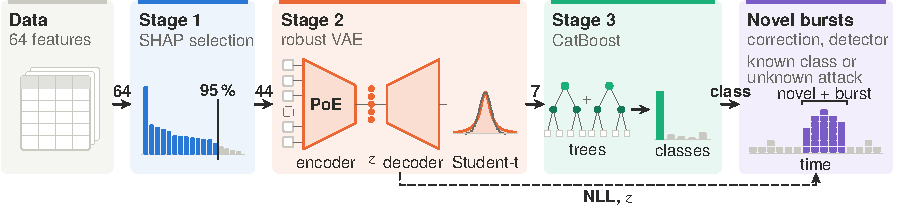
\includegraphics[width=\textwidth]{figures/architecture.pdf}
\Description{Diagram with five panels from left to right, joined by arrows labelled 64, 44, 7 and class. Data: a stack of flow tables with 64 features. Stage 1, SHAP selection: ranked importance bars, blue up to a vertical line marked 95 percent and grey after it. Stage 2, robust VAE: input boxes, one of them dashed, feed a trapezoid encoder labelled PoE, five latent units z, a trapezoid decoder, and a Student-t curve drawn over a dotted Gaussian. Stage 3, CatBoost: two symmetric trees added together, then five class-probability bars in which one bar is tall. Novel bursts, correction and detector, output known class or unknown attack: a row of small squares over time, in which a tall purple cluster in the middle is marked novel plus burst. A dashed arrow labelled NLL, z runs from the VAE to this panel.}
\caption{Architecture: Stage~2 encodes the defined features with a product of per-feature experts (PoE; an undefined statistic, dashed, is left out). In Stage~3, the correction relabels bursts of novel flows from the VAE NLL and latent mean $z$, and the detector checks the remaining Benign flows.}\label{fig:architecture}
\end{figure}

\subsection{Stage 1: CatBoost with SHAP Feature Selection}

Stage~1 ranks the 64 candidate features by mean absolute SHAP value~\cite{lundberg2017} across 20 CatBoost runs, each on a random 70\,\% of the features, and retains the smallest top set holding 95\,\% of the importance: 44 features on our data (Fig.~\ref{fig:shap}, Table~\ref{tab:settings}).

\subsection{Stage 2: Robust Variational Autoencoder}

Each part of our VAE~\cite{kingma2014} addresses a property of flow statistics.

\paragraph{Undefined Statistics.}
When a flow statistic cannot be calculated---such as an inter-arrival time on a single-packet flow or an idle time when no pause occurs---CICFlowMeter outputs a default 0~\cite{cicflowmeter}. These zeros represent missing data rather than measurements; in the training rows, \UndefinedIdleMax\,\% of \emph{Idle Max} entries and \UndefinedFlowIatStd\,\% of \emph{Flow IAT Std} entries are undefined. We follow the CICFlowMeter source code to flag these entries as missing ($b_j=0$). Each feature $j$ has its own small encoder, an expert, mapping $x_j$ to a Gaussian $\mathcal{N}(\mu_j,\sigma_j^2)$ over the latent vector $z\in\mathbb{R}^5$. The posterior is the product of the defined-feature experts and a standard normal prior expert~\cite{wu2018}: $\sigma^{-2}=1+\sum_j b_j\sigma_j^{-2}$ and $\mu=\sigma^{2}\sum_j b_j\sigma_j^{-2}\mu_j$. Thus, a missing feature neither affects the posterior nor adds a likelihood term~\cite{ma2019eddi,ivanov2019}.

\paragraph{Heavy Tails.}
Training flow durations vary across six orders of magnitude and forward packet counts across four, so a few extreme outliers dominate a standard Gaussian likelihood. The decoder therefore assigns each feature a Student-t likelihood with learned location, scale, and degrees of freedom~\cite{takahashi2018}, with negative log-likelihood $\ell_j$. A soft lower bound on the log scale prevents the scale from collapsing~\cite{rybkin2021}.

\paragraph{Neighbourhoods.}
Stage~3's burst correction counts flows in latent grid cells, which requires similar traffic to map to nearby latent coordinates---a property that the standard VAE objective does not enforce. We therefore add the 0-dimensional topological loss $\mathcal{L}_t$ of Moor et al.~\cite{moor2020}, comparing the minimum spanning trees of the inputs and posterior means within each batch.

\paragraph{Objective.}
To train the experts on incomplete rows, each batch also includes a second view $x_s$ per row that retains a random subset $s$ of the defined features~\cite{ma2019eddi,ivanov2019}. The VAE minimizes
\begin{multline}
\mathcal{L}=\sum_{v\in\{x,x_s\}}\Big(\mathbb{E}_{q(z\mid v)}\big[\textstyle\sum_j m^{v}_j\ell_j\big]+\beta\,\mathrm{KL}\big(q(z\mid v)\,\|\,p(z)\big)\Big)\\
+0.1\beta\,\mathrm{KL}\big(q(z\mid x_s)\,\|\,q(z\mid x)\big)+\gamma\mathcal{L}_t,
\end{multline}
where $m^v_j$ is 1 for features present in view $v$, $p(z)=\mathcal{N}(0,I)$, and the third term aligns the two views~\cite{sinha2021}. The weight is $\gamma=\topoweight$ (Sect.~\ref{sec:selection}).

\subsection{Stage 3: Classification, Correction and Detection}

\paragraph{Classifier.}
For each flow, the VAE produces seven outputs: the five posterior means $\mu$, the KL term, and the reconstruction NLL at $z=\mu$, summed over the \AlwaysDefinedCount\ features defined for every flow so that the sum has the same terms across flows. A multiclass CatBoost classifier~\cite{prokhorenkova2018} with balanced class weights predicts the class from these outputs and is tuned with Optuna~\cite{akiba2019}. Since the classifier outputs only training labels, evaluations on unseen attack families treat any non-Benign prediction as a detected attack, following the binary convention of~\cite{ferreira2020}.

\paragraph{Novel-Burst Correction.}
A learned attack can recur in a form the classifier misses: Slowloris teardown flows appear Benign to the classifier, yet look unusual to the VAE and arrive in bursts. The correction identifies such flows in three steps. First, a flow is \emph{novel} if its reconstruction NLL exceeds the $q_n$ quantile of Benign NLLs on a calibration day. Second, a flow lies in a \emph{burst} when many flows have recently arrived in its latent cell: after scaling each latent dimension by its training SD, the cell is the grid cube of side $w$ that contains the flow's posterior mean. Since the flow records carry no IP addresses, MIDAS-R~\cite{bhatia2020} takes the latent cell in place of a host pair, and a burst is flagged when its score exceeds the $q_b$ quantile of Benign training flows. Third, a flow that is both novel and in a burst takes the attack class predicted most often by the classifier among earlier flows from the last $W$ seconds of the same day, if that class count exceeds a support threshold; otherwise its prediction stands. The calibration day has no training attack classes, so any attack prediction on its Benign flows is a false alarm, and the $q_s$ quantile of these false-alarm counts sets the threshold. Every step uses only earlier flows, so the correction runs online. In the hold-out evaluation, same-day training flows stay in the stream as Benign predictions, so no training label adds attack support.

\paragraph{Unseen-Attack Detector.}
A flow from an unseen family that triggers no known-class prediction remains Benign after the correction, so a second CatBoost model, the detector, checks every remaining Benign flow. As days differ in their normal NLL level, its first input is the \emph{relative NLL}: the reconstruction NLL minus the running median NLL of earlier non-burst flows of the same day. The other four inputs are the KL term, the latent cell's MIDAS-R score, that score over novel flows only (relative NLL above its $q_n$ quantile on calibration-day Benign flows), and the share of novel flows in the cell over the last $W$ seconds. Converting each input to its percentile rank among Benign reference flows puts all days on one scale. Monotone constraints~\cite{incer2018} ensure that a larger input never lowers the attack score, so a more unusual flow never scores lower, and make it harder for the trees to learn a narrow value range of one training family.

Its positives are labelled attacks from families absent from the VAE and classifier training labels: the training rows of the left-out class in each leave-one-attack-out fold, encoded by that fold's models, plus the attacks of day 02-28 and further capture days (Sect.~\ref{sec:protocol}). The negatives are half of the Benign flows from these days and the calibration day, with the cut-off set for 1\,\% false alarms on the other half. A left-out day excludes that day and its families on all days from detector training; a fold excludes its class. Any flagged flow becomes an \emph{unknown attack}, a wrong class in the seen-class metrics.

\subsection{Hyperparameter Selection}\label{sec:selection}

No model weight or threshold is fitted on the hold-out or test day, and the VAE stops on the 02-28 ELBO. The topological weight $\gamma$ and the five correction settings are chosen with seed~3 on an inner split holding out the latest 20\,\% of training rows per day and class. The weight $\gamma$ maximizes mean per-class F1 with the correction at its start values. The correction settings are then tuned one by one to maximize mean attack-versus-Benign F1 across three leave-one-attack-out folds of the inner split. For the detector, the NLL is taken relative to either the calibration-day median NLL or the day's running median, and the inputs are chosen from five subsets; each configuration is validated by leaving out one further capture day or one fold at a time. The chosen configuration---the running median with all five inputs---achieves the highest mean detection rate among those with at most 2\,\% mean false alarms. Table~\ref{tab:settings} lists the grids and selected values.

\begin{table}[t]
\caption{Settings of the framework; Stage~3 values are search ranges of Optuna's TPE sampler.}\label{tab:settings}
\centering\scriptsize
\setlength{\tabcolsep}{3pt}
\begin{tabular}{L{1.5cm}L{10.27cm}}
\toprule
Part & Settings \\
\midrule
Stage 1 & 20 CatBoost runs on random 70\,\% feature subsets and $\le$50{,}000 training rows per class, SHAP on 1{,}000 rows per class; 300 iterations, depth 6, learning rate 0.1, balanced class weights \\
Stage 2 & all training rows; signed log, standardization on defined entries; 44 experts of 20 ReLU units, latent size 5; decoder 128 ReLU units, Student-t, soft bound $\log\hat\sigma\ge-6$, $\nu=1+\mathrm{softplus}$; $\beta=0.5$, consistency $0.1\beta$; second view: each defined feature kept with probability $1-\rho$, $\rho\sim U(0,0.7)$, and, in addition, the features removed that are undefined in a random other row of the batch; $\gamma\in\{0.1,0.3,1,3\}$, chosen $\gamma=\topoweight$, on 256 flows per batch, distances divided by their mean; Adam $8{\cdot}10^{-3}$, batch 32{,}768, $\le$1{,}000 epochs, learning rate halved after 3 flat epochs, stop after 10 epochs without a relative gain of $10^{-4}$ in the 02-28 ELBO \\
Stage 3 & CatBoost, plain boosting, balanced weights; Optuna TPE, 20 trials (10 random); iterations 200--1000, depth 4--8, learning rate 0.01--0.3, L2 1--30 (both log scale); mean per-class F1 over 3 time-blocked folds of a 10\,\% sample per day and class (classes under 2{,}000 rows whole); same search for raw CatBoost \\
Correction & grids, searched in this order from the start values in brackets: $w\in\{0.1,[0.2],0.5\}$, $q_b\in\{0.975,[0.99],0.995\}$, $W\in\{30,[60],120\}$\,s, $q_s\in\{0.975,[0.99],0.995\}$, $q_n\in\{0.90,0.95,[0.975],0.99\}$; chosen $w=\cellwidth$, $q_b=\burstq$, $W=\windowsec$\,s, $q_s=\supportq$, $q_n=\noveltyq$; latent axes divided by their training SD; MIDAS-R edge score only, decay 0.5~\cite{bhatia2020}, one-minute ticks; flows of the same second are not earlier than each other \\
Detector & CatBoost, depth 2, 500 iterations, learning rate 0.1, monotone; rank references: relative NLL and KL of calibration-day Benign flows, stream inputs of Benign training flows; median NLL of a reservoir sample of $\le$20{,}000 earlier flows of the day with MIDAS-R below its 0.9 Benign training quantile, refreshed every 500 flows (calibration-day median for the first 1{,}000); $\le$200{,}000 negatives per day; 1\,\% false alarms \\
\bottomrule
\end{tabular}
\end{table}

%-------------------------------------------------------------------------
\section{Experiments and Results}\label{sec:experiments}

\subsection{Dataset and Protocol}\label{sec:protocol}

We used the official CSE-CIC-IDS2018 CSV files~\cite{cic2018page,sharafaldin2018}, corrected their 12-hour CICFlowMeter timestamps~\cite{cicflowmeter}, and removed rows with non-finite values. To avoid shortcut features, we removed the timestamp~\cite{engelen2021,flood2024}, the destination port~\cite{dhooge2022}, \ConstantCount\ zero-variance columns, and three TCP header fields that identify the attacker hosts on the training days (\emph{Init Fwd Win Byts}, \emph{Init Bwd Win Byts}, \emph{Fwd Seg Size Min}; similar shortcuts are noted in~\cite{flood2024,engelen2021}), leaving 64 candidate features. Exact duplicates, rows from other days that match training rows, and label conflicts (identical feature vectors with different labels) were also filtered out; the conflicts include \FtpConflictRows\ FTP brute-force rows, consistent with the failed FTP attack reported in~\cite{liu2022error}.

Table~\ref{tab:data} details the resulting splits. Test day 02-21 contains only attack families excluded from training and thus serves as our unseen-family test. Its HOIC window includes a single-template burst of \BurstRows\ Benign flows; since Liu et al.~\cite{liu2022error} found no HOIC labelling error beyond a time offset, we retained these flows as Benign. Only \TestBenignOutside\ Benign flows of that day occur outside this burst. The detector also trains on further capture days in which at least six distinct hours each contain at least 1\,\% of the day's Benign flows, a rule that excludes the truncated file of day 02-16. On day 02-20, we removed \MislabelledUdpRows\ UDP flows labelled LOIC-HTTP within the LOIC-UDP window, since LOIC-UDP is a test-day class.

\begin{table}[t]
\caption{Data splits after cleaning: the hold-out contains the latest 20\,\% of each day and class.}\label{tab:data}
\centering\scriptsize
\setlength{\tabcolsep}{3pt}
\begin{tabular}{L{3.25cm}L{1.6cm}L{6.35cm}}
\toprule
Split (use) & Day(s) & Rows (class counts) \\
\midrule
\inputrows{tab_data_rows}
\bottomrule
\end{tabular}
\end{table}

\paragraph{Metrics and Runs.}
Seen classes are scored by the mean per-class F1 over the classes with at least 30 hold-out rows; the 8-row FTP class is reported separately. On unseen families, we measure the detection rate (DR), the Benign false-positive rate (FPR), and Youden's $J=\mathrm{DR}-\mathrm{FPR}$. Stage~1 runs once on the main split and once per fold, whereas every later model and threshold is retrained for each seed (3, 4, 5). Results give the mean and standard deviation (SD) over seeds and a paired bootstrap of the difference to raw CatBoost~\cite{koehn2004}.

\paragraph{Comparison Methods.}
Ten methods from related work---the \emph{re-run methods}---were trained on the same 44 Stage~1 features, rows, and seeds (Table~\ref{tab:baselines}), with class-balanced weights or batches and no synthetic oversampling. Each is evaluated on the hold-out, the test day, and the further days, and is retrained without the left-out class in each fold.

\begin{table}[t]
\caption{Re-run methods (top; deviations from the source in italics; not given: absent from the source) and reported results of related work (bottom; other splits and metrics). LOAO: leave-one-attack-out}\label{tab:baselines}\label{tab:literature}
\centering\scriptsize
\setlength{\tabcolsep}{2.5pt}
\begin{tabular}{L{2.4cm}L{9.2cm}}
\toprule
Method & Settings \\
\midrule
Random forest~\cite{sakr2026} & scikit-learn defaults, as the source; standardization; \emph{signed log, balanced class weights} \\
MLP~\cite{ferreira2020} & 24 hidden units (WEKA rule of the source code); \emph{scikit-learn with early stopping, not WEKA} \\
XGBoost~\cite{chen2016}, LightGBM~\cite{ke2017} & library defaults, signed log + standardization (XGBoost has no random step) \\
IDAE-XG~\cite{kang2022} & as the source; top 22 features by forest rank, 20 epochs (not given); \emph{multiclass; no upsampling} \\
CNN-1D~\cite{donoso2026} & as the source ($\le$20 epochs, patience 4); \emph{our split, stratified random split in the source} \\
FlowTransformer~\cite{manocchio2024} & 8-flow windows (source code), 2 decoder blocks, learning rate of the source grid; \emph{multiclass} \\
TabM~\cite{gorishniy2025} & package defaults, settings of the source (patience 16); \emph{no tuning} \\
FT-Transformer~\cite{gorishniy2021} & default configuration and optimizer (patience 16); \emph{no tuning, no ensemble} \\
TabNet~\cite{zegarra2023} & Table~4 of the source, patience 20; learning rate 0.02 (library default; not given); \emph{no SMOTE} \\
\midrule
Work & Data; split; reported result \\
\midrule
Ferreira~\cite{ferreira2020} & CSE-CIC-IDS2018, train 02-16, test 02-21; MLP TPR 0.898 on test attacks, 0 on LOIC-UDP \\
Sakr~\cite{sakr2026} & CSE-CIC-IDS2018, 9 days; random forest F1 0.957 (random split), 0.239 (LOAO mean) \\
Verkerken~\cite{verkerken2023} & CIC-IDS2017 random split: 41/47 unknown flows found; CSE-CIC-IDS2018 Infiltration recall 78.38\,\% \\
Soltani~\cite{soltani2021} & CSE-CIC-IDS2018 packet bytes, one unknown label per run: its accuracy 35.47--72.16\,\% \\
\bottomrule
\end{tabular}
\end{table}

\begin{figure}[t]
\centering
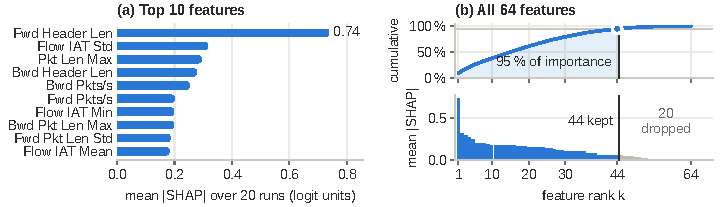
\includegraphics[width=\textwidth]{figures/shap_ranking.pdf}
\Description{Three panels. Left: horizontal bars of mean absolute SHAP for the top 10 of 64 features; Fwd Header Len leads at 0.74, followed by Flow IAT Std, Pkt Len Max, Bwd Header Len and Bwd Pkts/s near 0.25 to 0.32 and the rest near 0.18 to 0.20. Right top: cumulative share of importance against feature rank, reaching 95 percent at rank 44, marked by a vertical line. Right bottom: mean absolute SHAP of all 64 features by rank; the 44 kept features are blue and the 20 dropped features are grey.}
\caption{Stage 1 SHAP ranking: (a) mean $|$SHAP$|$ of the top 10 features over 20 runs; (b) cumulative share and importance of all 64 features (the 95\,\% rule keeps $k=44$). Splitting the 20 runs into two disjoint halves yields a Spearman rank correlation of \StabilitySpearman\ and a top-44 Jaccard index of \StabilityJaccard.}\label{fig:shap}
\end{figure}

\subsection{Seen Classes: The Correction on VAE Signals Gives the Gain}

We first compare the framework with a CatBoost model trained directly on the same 44 Stage~1 features (raw CatBoost) on the four seen classes with at least 30 hold-out rows (Table~\ref{tab:main}). The framework achieves a mean per-class F1 of \pmsd{\OursMean}{\OursSd}, above raw CatBoost (\pmsd{\RawMean}{\RawSd}) and the best re-run method (\BestBaselineMean). Across seeds 3, 4, and 5, the gain over raw CatBoost ranges from \GainMin\ to \GainMax, with 95\,\% paired bootstrap intervals of \BootstrapIntervals. Enabling the detector lowers the F1 only slightly, to \pmsd{\DetectorMean}{\DetectorSd}, because about 1\,\% of the Benign hold-out flows are flagged as unknown attacks. As Table~\ref{tab:perclass} shows, the gain stems from Slowloris, whereas raw CatBoost performs better on the 8-row FTP class and therefore over all five classes (\AllClassRaw\ versus \AllClassOurs).

The ablations in Table~\ref{tab:main} isolate the source of this gain. Without the correction, the VAE-fed classifier trails raw CatBoost (\NoCorrMean\ versus \RawMean). The correction raises its Slowloris recall from \SlowRecallBase\ (not tabulated) to \SlowRecallCorr, and the same VAE-driven correction lifts raw CatBoost to \RawCorrMean\ as well, tying the framework within the seed spread. However, raw CatBoost with the correction still runs the VAE for the NLL and latent cells, relabels more Benign flows, and is slower than the framework. The gain thus comes from the correction, which needs the VAE signals, not from the VAE as a feature compressor. Accordingly, a Gaussian instead of the Student-t likelihood, no topological loss, or the latent means alone change the F1 by at most \VaePartGap\ with the correction active, within the seed spread, whereas without the correction the topological loss lowers the F1. On unseen families, a detector on the VAE without the topological loss reaches a $J$ of \JArmBase\,\% on left-out days, against \JArmTopology\,\% with it, when both train on the further days only, so the loss does not change detection either. LightGBM or XGBoost in Stage~3 give a similar F1 but a lower balanced accuracy. Concatenating the 44 raw features with the seven VAE outputs still trails raw CatBoost before the correction (\ConcatNoCorrMean\ versus \RawMean), ties the framework after it (\ConcatMean), and removes the FTP false alarms (FTP F1 \ConcatFtpScore\ versus \OursFtpScore).

\paragraph{Inference Time.} On a single CPU thread, end-to-end processing with the detector takes 0.050\,ms per flow, compared to 0.018\,ms for raw CatBoost: the fused VAE and CatBoost graph accounts for 0.044\,ms (0.046\,ms as two separate graphs), the correction takes 0.00015\,ms, and the detector takes 0.0058\,ms. We timed each pipeline with a time in Table~\ref{tab:main} as ONNX Runtime 1.31 graphs and C++ code on one thread of an Intel Core Ultra 9 275HX, one flow per call from the extracted features to the final label, over the 100{,}000 consecutive flows in the middle of day 02-21 (98{,}562 Benign burst and 1{,}438 attack flows). Each time is the median of 4 passes; a full repeat gave the same order of the 16 pipelines and a framework time 1.3\,\% higher.


\begin{table}[t]
\caption{Hold-out mean per-class F1 (classes $\ge$30 rows) per seed and mean $\pm$ SD, balanced accuracy (all classes), Benign hold-out flows relabelled (sum over seeds; with the detector: by the correction and the detector), and CPU ms per flow (batch 1, one thread, seed 3). With the correction, the framework has a higher mean F1 than raw CatBoost and each re-run method.}\label{tab:main}
\centering\scriptsize
\setlength{\tabcolsep}{2.2pt}
\begin{tabular}{L{3.3cm}ccccccc}
\toprule
Configuration & Seed 3 & Seed 4 & Seed 5 & Mean F1 & Bal.\ acc. & Relab. & ms/flow \\
\midrule
\inputrows{tab_main_rows}
\bottomrule
\end{tabular}
\end{table}

\begin{table}[t]
\caption{Per-class hold-out results, mean over seeds 3--5, of the framework and raw CatBoost (top), and the confusion matrix of the framework, seed 3 (bottom; rows: true class)}\label{tab:perclass}\label{tab:confusion}
\centering\scriptsize
\setlength{\tabcolsep}{4pt}
\begin{tabular}{lrcccccc}
\toprule
 & & \multicolumn{3}{c}{Ours (with correction)} & \multicolumn{3}{c}{Raw CatBoost (44 features)} \\
\cmidrule(lr){3-5}\cmidrule(lr){6-8}
Class & Rows & Precision & Recall & F1 & Precision & Recall & F1 \\
\midrule
\inputrows{tab_perclass_rows}
\bottomrule
\end{tabular}

\smallskip
\begin{tabular}{lrrrrr}
\toprule
True $\backslash$ predicted & Benign & GoldenEye & Slowloris & FTP & SSH \\
\midrule
\inputrows{tab_confusion_rows}
\bottomrule
\end{tabular}
\end{table}

Table~\ref{tab:featurecount} measures F1 and cost with the $k$ most important features of Stage~1 (seed~3; $k=64$: all 79 columns minus the 15 dropped); for $k>10$, our F1 stays within 0.9870--0.9908, and $k\in\{23, 40, 64\}$ score above the $k=44$ of the 95\,\% rule.

\begin{table}[t]
\caption{Feature-count ablation (seed 3): hold-out mean per-class F1, VAE training time in s (one VAE at a time on the GPU) and inference time in ms per flow (batch 1, one thread, no detector, as Table~\ref{tab:main})}\label{tab:featurecount}
\centering\scriptsize
\setlength{\tabcolsep}{3pt}
\begin{tabular}{rcccrcc}
\toprule
 & \multicolumn{3}{c}{F1} & & \multicolumn{2}{c}{ms per flow} \\
\cmidrule(lr){2-4}\cmidrule(lr){6-7}
$k$ & Ours & Raw & Raw + corr. & VAE (s) & Ours & Raw \\
\midrule
10 & 0.9738 & 0.9815 & 0.9881 & 141 & 0.046 & 0.017 \\
15 & 0.9877 & 0.9792 & 0.9886 & 158 & 0.072 & 0.019 \\
23 & 0.9908 & 0.9782 & 0.9895 & 273 & 0.051 & 0.015 \\
30 & 0.9870 & 0.9799 & 0.9908 & 357 & 0.054 & 0.024 \\
40 & 0.9902 & 0.9813 & 0.9911 & 302 & 0.061 & 0.019 \\
\textbf{44} & 0.9883 & 0.9800 & 0.9911 & 317 & 0.044 & 0.018 \\
64 & 0.9908 & 0.9805 & 0.9906 & 392 & 0.057 & 0.016 \\
\bottomrule
\end{tabular}
\end{table}


\subsection{Unseen Attack Families}\label{sec:unseen}
\begin{table}[t]
\caption{Attack families absent from all training labels, in \%, mean $\pm$ SD over seeds 3--5: (a) left-out days, DR and Benign FPR of the detector alone; (b) leave-one-attack-out folds, DR on days 02-14 and 02-15 after each step, and hold-out Benign FPR; with raw CatBoost as classifier (same correction and detector), the mean final DR is 0.01 to 1.67 points higher per fold.}\label{tab:detectordays}\label{tab:loo}
\centering\scriptsize
\setlength{\tabcolsep}{1.5pt}
\renewcommand{\pmsd}[2]{#1$\pm$#2}
\begin{minipage}[t]{0.4\textwidth}\centering
(a) Left-out days\\[2pt]
\begin{tabular}{llcc}
\toprule
Day & Family & DR & FPR \\
\midrule
02-28 & Infiltration & \pmsd{2.34}{1.83} & \pmsd{2.42}{0.23} \\
02-20 & LOIC-HTTP & \pmsd{50.06}{0.12} & \pmsd{0.91}{0.16} \\
02-22 & Web brute force & \pmsd{30.84}{21.21} & \pmsd{0.61}{0.06} \\
 & SQL injection & \pmsd{13.04}{7.53} &  \\
 & XSS & \pmsd{48.44}{17.61} &  \\
03-01 & Infiltration & \pmsd{3.03}{0.71} & \pmsd{0.68}{0.01} \\
03-02 & Bot & \pmsd{68.24}{2.06} & \pmsd{0.68}{0.04} \\
\bottomrule
\end{tabular}
\end{minipage}\hfill
\begin{minipage}[t]{0.595\textwidth}\centering
(b) Leave-one-attack-out folds\\[2pt]
\begin{tabular}{lcccc}
\toprule
Removed class & Classifier & + corr. & + det. & FPR \\
\midrule
SSH-BruteForce & \pmsd{0.0007}{0.001} & \pmsd{0.0007}{0.001} & \pmsd{95.16}{5.02} & \pmsd{2.19}{1.21} \\
DoS GoldenEye & \pmsd{0.11}{0.01} & \pmsd{11.96}{1.40} & \pmsd{58.19}{19.27} & \pmsd{1.68}{0.92} \\
DoS Slowloris & \pmsd{53.01}{13.28} & \pmsd{71.09}{2.01} & \pmsd{87.43}{8.32} & \pmsd{2.03}{0.97} \\
\bottomrule
\end{tabular}
\end{minipage}
\end{table}

\begin{table}[t]
\caption{Unseen attack families, in \%, mean over seeds 3--5: Youden's $J$ is the detection rate (DR) minus the Benign false-positive rate (FPR); a re-run method flags a flow whose argmax class is not Benign. $^+$: trained also on the further days and flagged at the detector's cut-off. Left-out days: mean over day and family; folds: mean over the three folds. Test day 02-21: DR, Benign FPR outside and inside the burst, and $J$ against all Benign flows.}\label{tab:unseen}
\centering\scriptsize
\setlength{\tabcolsep}{3pt}
\begin{tabular}{L{2.6cm}cccccccc}
\toprule
 & \multicolumn{2}{c}{$J$} & \multicolumn{6}{c}{Test day} \\
\cmidrule(lr){2-3}\cmidrule(lr){4-9}
 & Left-out days & Folds & DR UDP & DR HOIC & FPR out & FPR burst & $J$ UDP & $J$ HOIC \\
\midrule
\textbf{Ours + detector} & 30.27 & 78.29 & 81.35 & 0.01 & 15.42 & 66.77 & 14.88 & $-$66.46 \\
\midrule
Random forest~\cite{sakr2026} & 0.03 & 15.81 & 0 & 0 & 0.27 & 0.0003 & $-$0.002 & $-$0.002 \\
MLP~\cite{ferreira2020} & 1.60 & 18.99 & 0 & 0 & 0.72 & 4.05 & $-$4.03 & $-$4.03 \\
XGBoost~\cite{chen2016} & $-$0.01 & 23.90 & 0 & 0 & 0.38 & 0 & $-$0.002 & $-$0.002 \\
LightGBM~\cite{ke2017} & $-$0.01 & 5.36 & 0.15 & 0 & 0.35 & 0.00009 & 0.15 & $-$0.002 \\
IDAE-XG~\cite{kang2022} & 24.57 & 36.52 & 99.81 & 32.17 & 68.17 & 67.64 & 32.16 & $-$35.48 \\
CNN-1D~\cite{donoso2026} & 0.60 & 16.56 & 0.02 & 0 & 0.49 & 20.57 & $-$20.43 & $-$20.45 \\
FlowTransformer~\cite{manocchio2024} & 8.33 & 8.02 & 93.29 & 17.32 & 38.35 & 68.57 & 24.90 & $-$51.07 \\
TabM~\cite{gorishniy2025} & 0.02 & 16.84 & 63.91 & 0 & 1.36 & 0.57 & 63.34 & $-$0.57 \\
FT-Transformer~\cite{gorishniy2021} & 0.31 & 20.85 & 6.61 & 0 & 0.64 & 0.94 & 5.67 & $-$0.94 \\
TabNet~\cite{zegarra2023} & 0.07 & 16.94 & 0 & 0.23 & 0.53 & 25.01 & $-$24.87 & $-$24.64 \\
\midrule
Random forest$^+$ & 0.16 & $-$0.01 & 0 & 0.43 & 0.05 & 0 & $-$0.0003 & 0.43 \\
MLP$^+$ & 1.18 & 34.35 & 99.83 & 0.0002 & 1.38 & 27.43 & 72.55 & $-$27.27 \\
XGBoost$^+$ & 0.98 & 24.08 & 0 & 0.11 & 0.45 & 0 & $-$0.003 & 0.11 \\
LightGBM$^+$ & 6.05 & 22.96 & 0.50 & 0.33 & 0.28 & 0 & 0.50 & 0.33 \\
IDAE-XG$^+$ & $-$0.25 & 0.68 & 46.22 & 0.34 & 1.22 & 22.01 & 24.34 & $-$21.54 \\
Isolation Forest$^+$~\cite{liu2008} & 0.36 & $-$0.65 & 66.69 & 0 & 33.44 & 0.01 & 66.48 & $-$0.21 \\
\bottomrule
\end{tabular}
\end{table}


Table~\ref{tab:detectordays} tests the detector alone on left-out days and the framework with the detector in the leave-one-attack-out folds. The detector mainly catches families whose flows arrive as bursts of novel flows. For LOIC-HTTP, it flags \LoicRequestDetection\,\% of request flows but only \LoicNoReplyDetection\,\% of unanswered attempts, while Infiltration stays mostly undetected. The VAE-based inputs are key: a CatBoost detector on the 44 raw features instead of its five inputs, trained on the same rows with the same cut-off but without monotone constraints, flags on average only \RawDetectorDetection\,\% (depth 6) and \RawDetectorTwoDetection\,\% (depth 2) of each left-out family's flows, versus \DetectorAloneDetection\,\% for ours (mean of Table~\ref{tab:detectordays}a), showing that the labelled further days and tree depth alone do not explain the detection.

Table~\ref{tab:unseen} compares all methods by Youden's $J$. Trained on days 02-14 and 02-15 only, our classifier scores like most re-run methods ($J$ \JClassifierDays\,\% on left-out days); with the detector, also trained on the further days, the framework reaches \JOursDays\,\% and \JOursFolds\,\% in the folds. Since the detector configuration was selected on these days and folds (Sect.~\ref{sec:selection}), only the test day is unused by that choice. The test day shows the limit of the burst signal: 99.4\,\% of its Benign flows belong to one burst inside the HOIC window. The framework detects \TestUdpMean\,\% of LOIC-UDP flows, but also flags \TestBurstFprMean\,\% of this Benign burst, which receives higher detector scores than the HOIC flows. In the rows marked $^+$ in Table~\ref{tab:unseen}, the shallow re-run methods also train on the further days except the evaluated one, with each attack flow labelled by family, and flag flows by the detector's cut-off rule; Isolation Forest~\cite{liu2008}, an open-set detector, trains on their Benign flows only. Given the same days, the best reach $J$ \JEqualBestDays\,\% on left-out days (\JEqualBestDaysName) and \JEqualBestFolds\,\% in the folds (\JEqualBestFoldsName), versus \JOursDaysEqual\,\% and \JOursFoldsEqual\,\%.

\section{Limits}\label{sec:discussion}
Unusual Benign bursts can trigger false alarms, attacks that arrive without bursts give no signal, and the correction assumes a single dominant attack class per time window.
The evidence comes from three seeds on one dataset with known errors and label faults~\cite{engelen2021,liu2022error}. The deep re-run methods (CNN-1D, FlowTransformer, TabM, FT-Transformer, TabNet) were not trained on the further days, Kitsune~\cite{mirsky2018} was not run, the re-run methods use defaults without the correction, and the missing-entry handling was not ablated.

%-------------------------------------------------------------------------
\section{Conclusion}\label{sec:conclusion}

We proposed a hybrid VAE-CatBoost framework in which a robust VAE serves both a classifier and two streaming components. On CSE-CIC-IDS2018, the correction lifts the mean per-class F1 of the four larger classes above raw CatBoost and ten untuned re-run methods, and the framework with the detector reaches a Youden's $J$ of \JOursDaysEqual\,\% on left-out days, versus \JEqualBestDays\,\% for the best untuned re-run method given the same days. A large Benign burst on the test day defeats the detector; separating such bursts from attacks remains future work.

\begin{credits}
\subsubsection{Use of AI Tools.}
Claude Code was used for the implementation of the code and for finding bugs.

\subsubsection{\discintname}
The authors have no competing interests to declare that are relevant to the content of this article.
\end{credits}

\bibliographystyle{splncs04u}
\bibliography{refs}

\end{document}
